% !TeX root = Trafficsimulation_Documentation.tex

\chapter{Design}
\label{Design}

In diesem Kapitel werden die Implementierungen der einzelnen Komponenten sowie deren Schnittstellen zu anderen Komponenten dokumentiert.

% In diesem Kapitel das Design der Verkehrssimulation erklärt. Hier wird auf die wesentlichen Teile eingegangen, welche zum Erreichen der jeweiligen Ziele notwendig sind. 

% wos ghead hin?

\thispagestyle{standard}
\pagestyle{standard}

\section{Strassensystem}
\label{Strassensystem}

Das Strassensystem besteht aus drei Grundelementen den Ampeln, Strassen und Kreuzungen.

\subsection{Ampeln}

Die Ampeln wurden von uns als eigenständiges System geplant und umgesetzt. Um dieses Ziel zu erreichen erstellten wir zuerst auf Basis der Technologie TCP-Channel ein RemoteObject in Form einer eigenen DLL. Dieses RemoteObject definiert die Datenstrukturen, welche in weiterer Folge zwischen Client und Server geteilt werden. Als Serveranwendung erstellten wir eine Konsolenanwendung, welche wir auf einem öffentlich erreichbaren Linux Server mit Hilfe von Mono deployten. Als Clientgegenstellen für dieses System können verschiedene Unityinstanzen den Dienst der Serveranwendung verwenden. Sowohl am Client als auch am Server ist als DLL das RemoteObject hinterlegt. Instanzen des RemoteObjects können mit Hilfe am Server definierten Interfaces von den Clients erstellt und bearbeitet werden. Die somit erstellten Instanzen werden dann durch die TCP-Channel Technologie zwischen Client unser Server geteilt. Somit können Clients komfortabel mit ihrem lokalen Stub des RemoteObjects arbeiten ohne die Komplexität der IPC mitzubekommen. 

Durch die zentrale Definition des RemoteObjects in Form einer DLL können die geteilten Datenstrukturen zentral erweitert und gewartet werden.

\subsection{Straßen}

Die Straßen sind jene Element auf denen sich die Fahrzeuge bewegen sollen. Dabei soll in diesen keine Logik enthalten sein, um der realen Welt nahe zu kommen und das System einfach zu halten. Es gibt unterschiedliche Typen von Straßenelementen. Dazu zählen Geraden und Kurven. Damit sich die Fahrzeuge auf den Straßen bewegen werden sogenannte Wegpunkte auf den Straßen platziert. Die Fahrzeuge fahren somit von einem zum nächsten Wegpunkt. In Kurven sind mehrere Wegpunkte nötig, um eine schöne Bewegung zu simulieren. Die Wegpunkte werden jeweils in eine positive und eine negative Richtung gesetzt für die beiden Fahrtrichtungen. Am Beginn jedes Straßenelements befindet sich ein Kollider, der dem Fahrzeug mitteilt, auf welcher Straßenseite er sich befindet.

\begin{figure}[H]
\begin{center}
	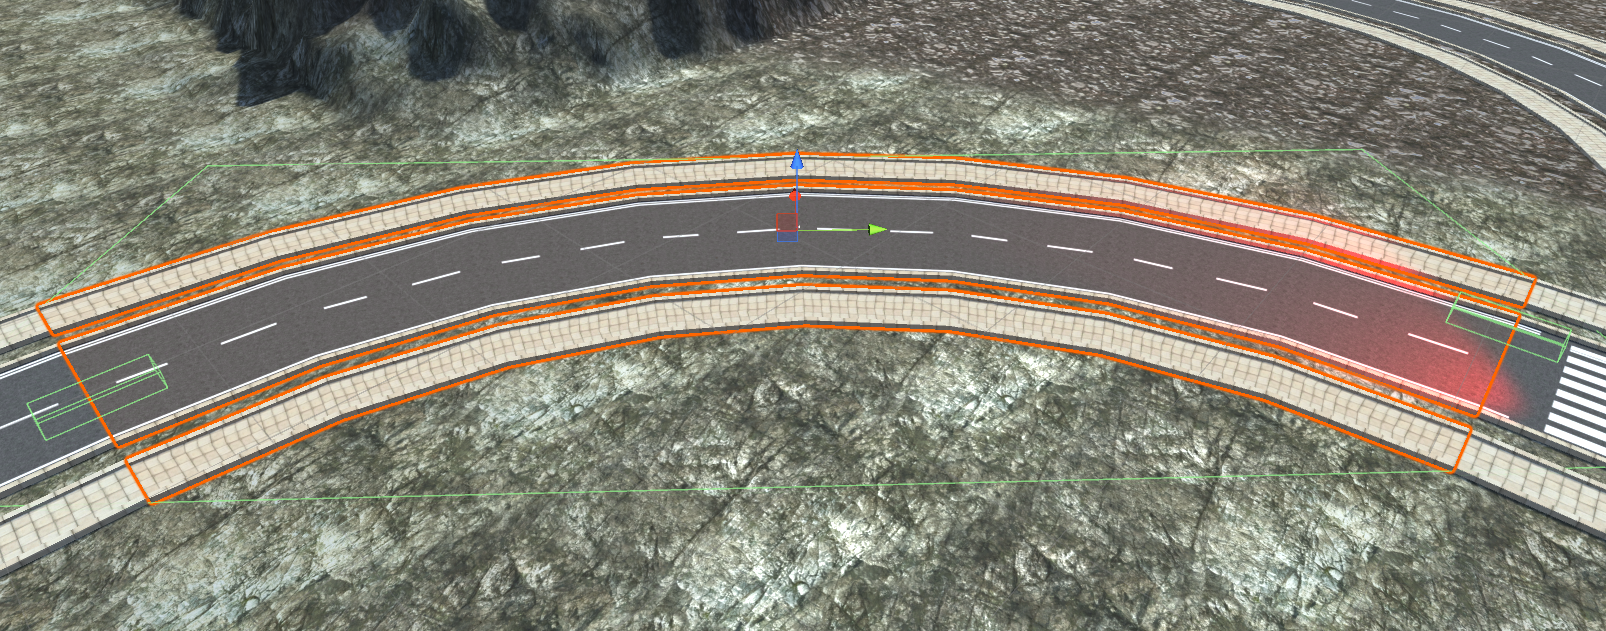
\includegraphics[width=1\textwidth]{BilderAllgemein/street_collider.png}
\end{center}
	\caption{Collider an normaler Straße}
	\label{img:street_collider}
\end{figure}

\subsection{Kreuzungen}

Die Kreuzungen unterscheiden sich in T- und X-Kreuzungen und werden auch nur mit der nötigsten Logik ausgestattet. Dabei kann beim erstellen zwischen geregelten und ungeregelten Kreuzungen unterschieden werden. Werden geregelte Kreuzungen erstellt, wird automatisch die Ampelsteuerung initialisiert und die Kreuzung regelt auch das Darstellen der Farben für die Ampeln. Weiters besitzt jede Kreuzung beim Einfahren einen Kollider um den Fahrzeugen mitzuteilen, dass sie sich einer Kreuzung nähren. Das Fahrzeug kann danach von der Kreuzung den Ampelstatus abfragen. Weiters erhält das Fahrzeug nachdem es sich für die neue Fahrtrichtung entschieden hat die neuen Wegpunkte und Strassenelemente für die Weiterfahrt.

\begin{figure}[H]
\begin{center}
	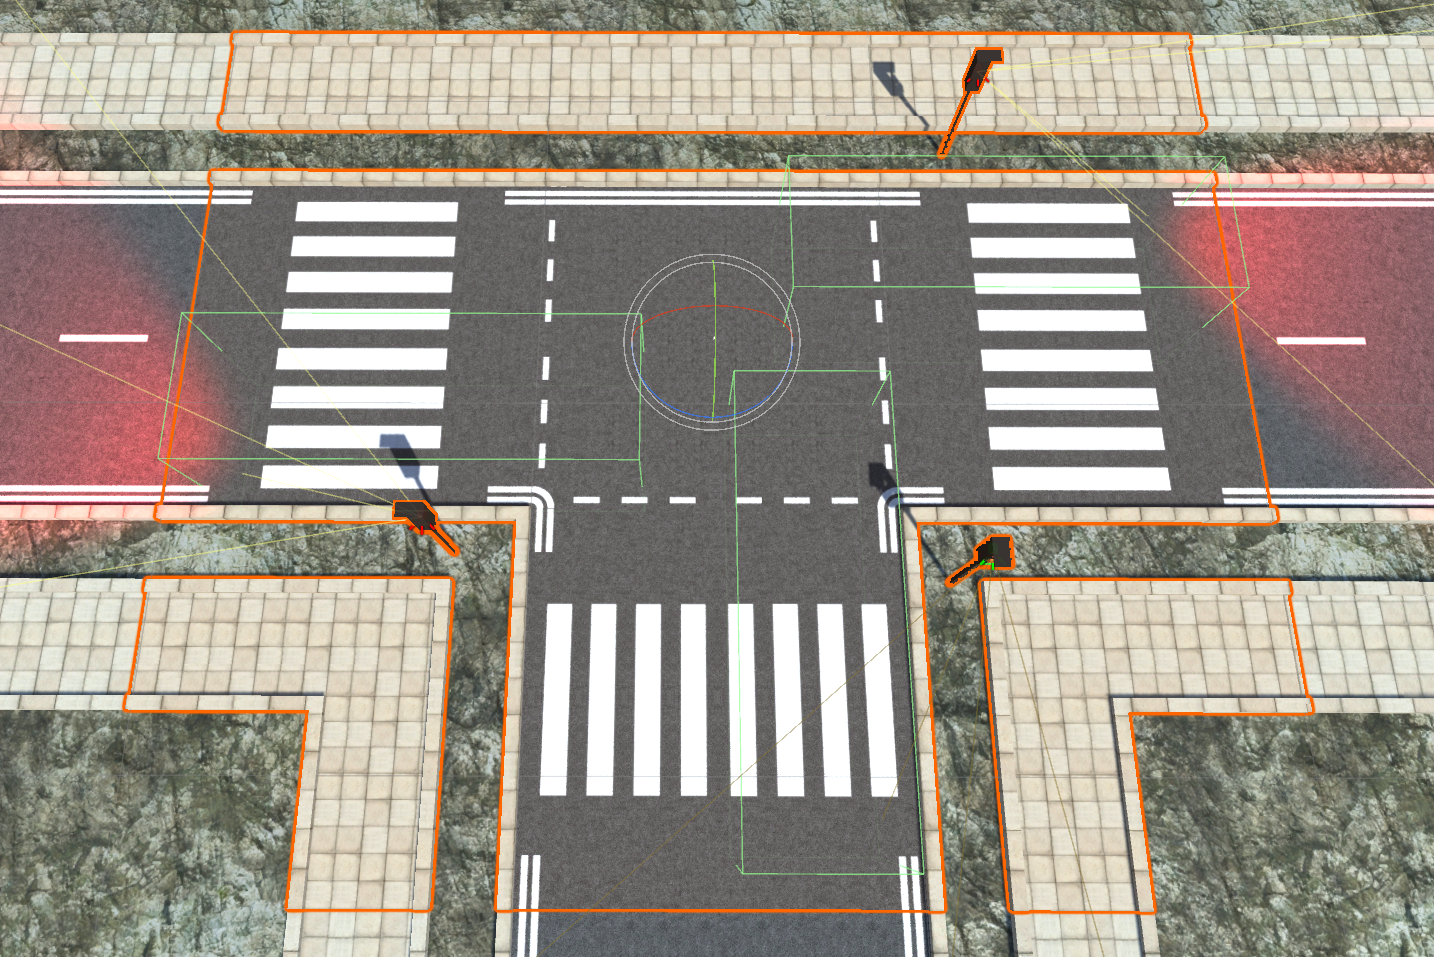
\includegraphics[width=1\textwidth]{BilderAllgemein/crossing_collider.png}
\end{center}
	\caption{Collider an Kreuzung}
	\label{img:crossing_collider}
\end{figure}

\subsection{Spawn}

Hier werden je nach Einstellung der Controls die Fahrzeuge gespawnt bzw despawnt, sobald sie mit dem in Abbildung \ref{img:spawn} gezeigten Collider in Berührung kommen.

\begin{figure}[H]
\begin{center}
	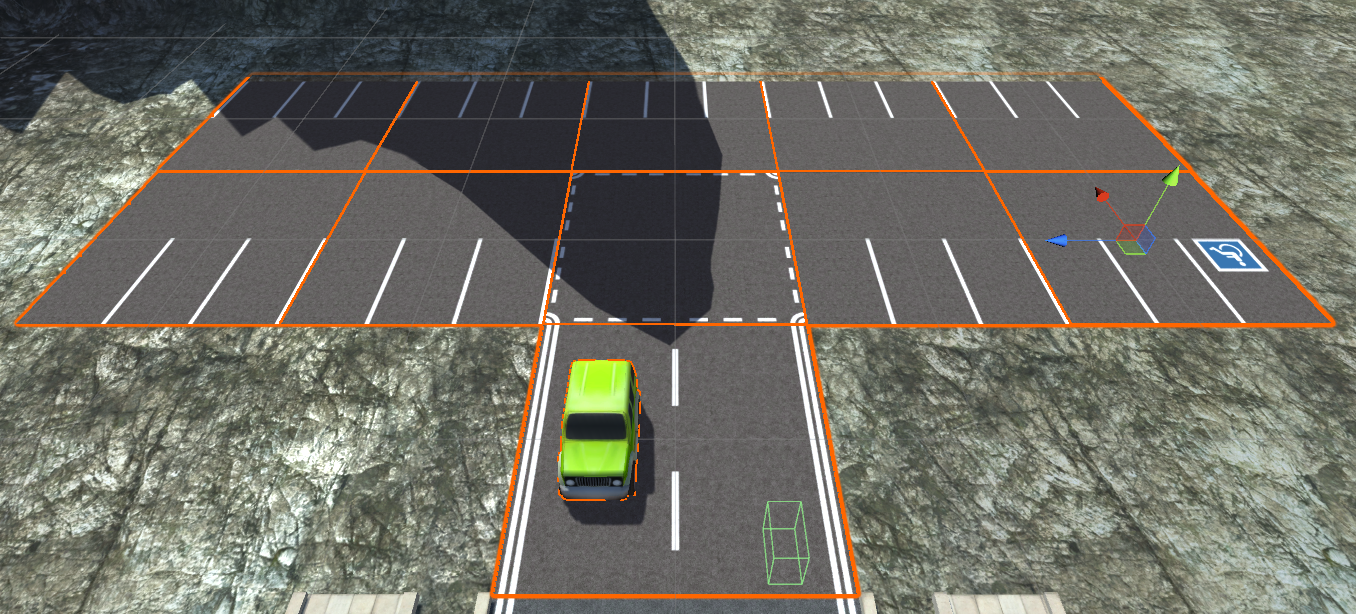
\includegraphics[width=1\textwidth]{BilderAllgemein/spawn.png}
\end{center}
	\caption{Spawn der Fahrzeuge}
	\label{img:spawn}
\end{figure}

\section{Fahrzeuglogik}
\label{Fahrzeuglogik}

Die Fahrzeuge implementieren alle ein Skript, welches für das Erkennen von Ampeln, Fahrzeugen und sonstiges Hindernissen zuständig ist. Dies ermöglicht eine völlige Kapselung und somit die Unabhängigkeit zur Straße und Kreuzung. Das bedeutet, dass Straßen und Kreuzungen nur sogenannte "Collider" zur Verfügung stellen, mit denen die Fahrzeuge interagieren können. Somit bleibt die gesamte Intelligenz in den Fahrzeugen.

Diese Collider werden je nach Geschwindigkeit des Fahrzeugs länger bzw. größer (wie in Abbildung \ref{img:car_collider} gezeigt) um somit auf Hindernisse wie andere Fahrzeuge, Kreuzungen und sonstiges frühzeitig reagieren zu können.

Das Erkennen und Verringern der Gschwindigkeit auf andere Fahrzeuge wird mittels Raycast erledigt. Die Lösung mit den Collidern war ein Problem, da sich die Fahrzeuge, nicht mehr bewegt haben, nachdem sie kollidiert sind.

\begin{figure}[H]
\begin{center}
	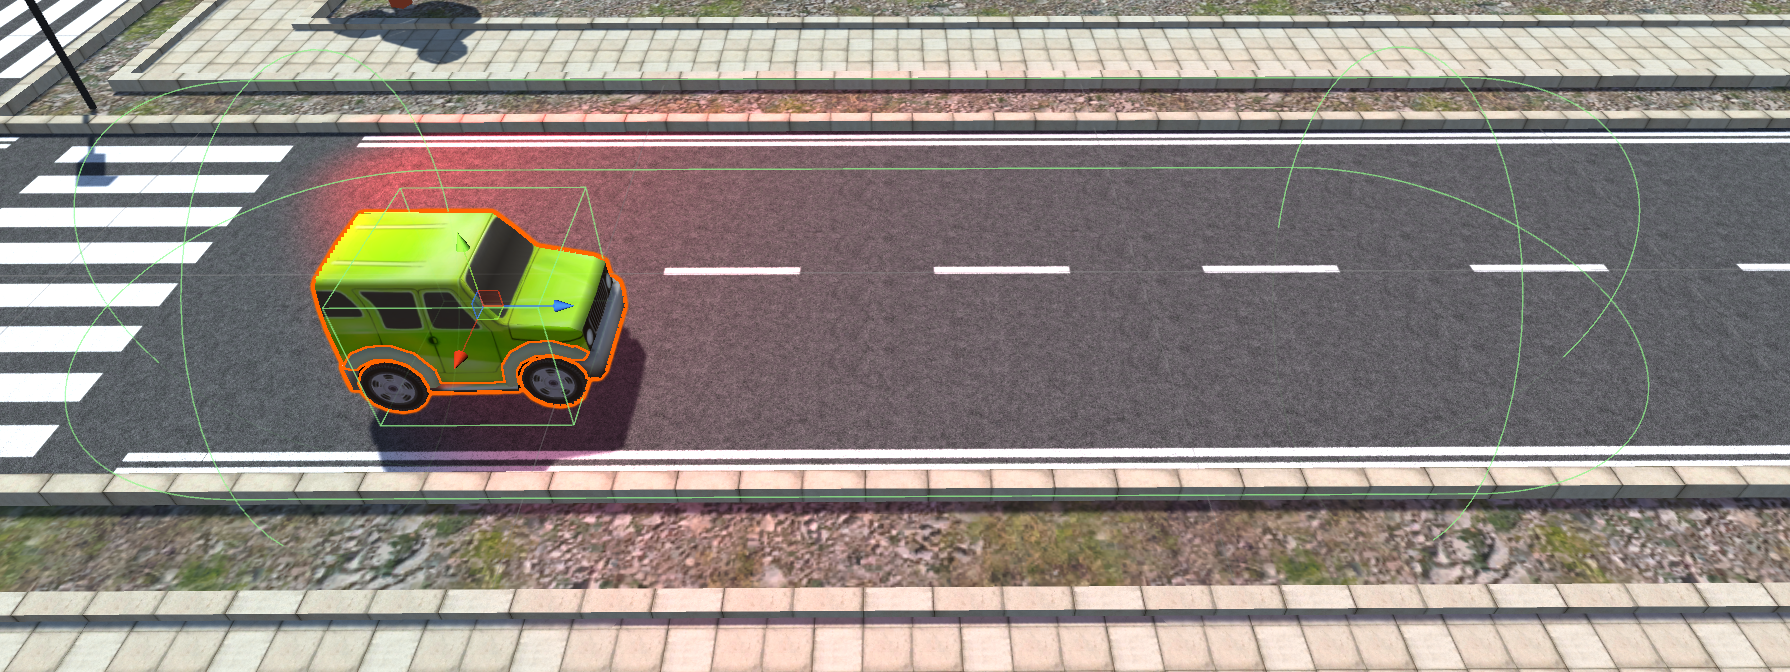
\includegraphics[width=1\textwidth]{BilderAllgemein/Jeep_Collider.png}
\end{center}
	\caption{Collider an Fahrzeugen}
	\label{img:car_collider}
\end{figure}


\section{Ampelsteuerung}

Die zentrale Komponente der Ampelsteuerung ist das RemoteObject. Wie bereits erwähnt handelt es sich dabei um eine eigenständige Komponente, welche in Form einer DLL in diverse Projekte leicht eingebunden und zentral gewartet werden kann. Das RemoteObject repräsentiert die Datenstrukturen und Funktionalitäten, welche zwischen Client und Server mit Hilfe der TCP-Channel Technologie geteilt werden.

Das RemoteObject bietet die Möglichkeit eine beliebige Anzahl von Kreuzungen zu erstellen und zu verwalten. Die Logik für den Aufbau der IPC-Verbindung wird dabei direkt im Client oder Server hinterlegt. Mit Hilfe von definierte Interfaces hat der Client die Möglichkeit Kreuzungen mit drei oder vier Ampeln am Server-Skeleton anzulegen. Die Kreuzungen werden entweder mit einer festgelegten Standardkonfiguration oder mit den vom Entwickler angegeben Übergabeparametern angelegt.

Von bereits angelegten Kreuzungen können die Zykluszeiten der einzelnen Ampeln editiert werden. Weiters ist es möglich das RemoteObject zu reseten und somit den Initialzustand wiederherzustellen.

Die einzelnen Kreuzungen, welche am RemoteObject angelegt sind können separat gestartet werden. Beim Starten einer Kreuzung wird ein eigener Thread für jede Ampel der Kreuzung erzeugt in dem eine Statemachine für die Ampelschaltung abläuft. Dieser Thread läuft bis entweder die Serveranwendung terminiert wird oder die Kreuzung durch einen Reset vom Client gelöscht wird. Die Statemachine einer Ampel durchläuft die üblichen Stati und berücksichtigt dabei die Konfiguration der entsprechenden Ampel. 

Mit Hilfe der ID einer Kreuzung und der Bezeichnung einer konkreten Ampel der Kreuzung kann der Status einer Ampel abgefragt werden.

Durch die Verwendung der TCP-Channel Technologie und der Definition des RemoteObjects in Form einer eigenen DLL wurde die Komplexität einer IPC sehr gut abstrahiert. Leider erfuhren wir während den Tests, dass die von uns verwendete Technologie sehr anfällig gegenüber schlechten Latenzzeiten ist. Dies wirkt sich in Form von Verbindungsproblemen zwischen Client und Server aus. Daher würde ich die Technologie TCP-Channel für IPC nur innerhalb eines lokalen Netzwerkes empfehlen.


\section{Hindernisse}
\label{Hindernisse}

Mit einem Klick der Maus sollen überall in der Welt Hindernisse platziert werden, welche anschließend von Fahrzeugen umfahren werden müssen. Durch einen weiteren Klick auf ein Hindernis soll dieses wieder gelöscht werden. 

Unity ermöglicht das Erstellen von GameObjects zur Laufzeit. Durch den Klick auf die Welt können die Koordinaten des Klicks festgestellt werden und somit das GameObject, welches bereits beim Start der Verkehrssimulation geladen wurde, platziert werden.

Durch das Halten eines Buttons auf der Tastatur soll die Erstellung von Hindernissen aktiviert werden. Dies verhindert, dass der Benutzer unbeabsichtigt zu viele Hindernisse erstellt.

\section{Aus- und Einfahren von Fahrzeugen anderer Gruppen}

Die Message Queue übernimmt die Kommunikation mit den anderen Gruppen. Die Kommunikation mit den anderen Gruppen wird über einen externen Server abgewickelt, auf denen sich die Gruppen anmelden und ihre Queues abonnieren können. Ein Format, basierend auf JSON wurde zwischen den Gruppenteilnehmern definiert.

Als Protokoll wird dabei AMPQ verwendet, der dazugehörende Server, RabbitMQ implementiert diese Protokoll und ermöglicht die Übertragung von Nachrichten.